%%%%%%%%%%%%%%%%%%%%%%%%%%%%%%%%%%%%%%%%%%%%%%%%%%%%%%%%%%%%%%%%%%%%%
% LaTeX Template: Project Titlepage Modified (v 0.1) by rcx
%
% Original Source: http://www.howtotex.com
% Date: February 2014
% 
% This is a title page template which be used for articles & reports.
% 
% This is the modified version of the original Latex template from
% aforementioned website.
% 
%%%%%%%%%%%%%%%%%%%%%%%%%%%%%%%%%%%%%%%%%%%%%%%%%%%%%%%%%%%%%%%%%%%%%%

\documentclass[11pt]{article}
\usepackage[a4paper]{geometry}
\usepackage[myheadings]{fullpage}
\usepackage{mathtools}
\usepackage{fancyhdr}
\usepackage{lastpage}
\usepackage{graphicx, wrapfig, subcaption, setspace, booktabs}
\usepackage[T1]{fontenc}
\usepackage[font=small, labelfont=bf]{caption}
\usepackage{fourier}
\usepackage[protrusion=true, expansion=true]{microtype}
\usepackage[english]{babel}
\usepackage{sectsty}
\usepackage{url, lipsum}
\usepackage{natbib}
\usepackage{bibentry}
\usepackage{booktabs}
\usepackage{pdflscape}
\newcommand{\HRule}[1]{\rule{\linewidth}{#1}}
% \renewcommand{\contentsname}{"Table of Contents"}
\addto\captionsenglish{% Replace "english" with the language you use
  \renewcommand{\contentsname}%
    {Table of Contents}%
}
\onehalfspacing
\setcounter{tocdepth}{4}
\setcounter{secnumdepth}{5}


%-------------------------------------------------------------------------------
% HEADER & FOOTER
%-------------------------------------------------------------------------------
\pagestyle{fancy}
\fancyhf{}
\setlength\headheight{15pt}
\fancyhead[L]{Group K}
\fancyhead[R]{IT University of Copenhagen}
\fancyfoot[R]{Page \thepage\ of \pageref{LastPage}}
%-------------------------------------------------------------------------------
% TITLE PAGE
%-------------------------------------------------------------------------------
\bibliographystyle{unsrt}
\begin{document}

% \bibliography{bib.bib}
\title{ \normalsize \textsc{First Year Project - BSFIYEP1KU}
		\\ [2.0cm]
		\HRule{0.5pt} \\
		\LARGE \textbf{\uppercase{COVID-19 and the Weather}\\
		\normalsize{\textsc{SUBTITLE}}}
		\HRule{2pt} \\ [0.5cm]
		\normalsize \today \vspace*{5\baselineskip}}

\date{}

\author{
		\textbf{Group K} \\ 
		Andreas Magnus Benggaard - andbe@itu.dk\\ 
		Michal Rynowiecki - miry@itu.dk\\ 
		Nicolai Jacob Kofod-Jensen - nkof@itu.dk\\ 
		Sam Younes isyo@itu.dk \\ 
		Sree Keerthi Desu - srde@itu.dk}
		% \hline
		% Exam Number: 4\\
		% Character Count: \\
		% IT University of Copenhagen \\

\maketitle
\newpage

\tableofcontents
\newpage

%-------------------------------------------------------------------------------
% Section title formatting
\sectionfont{\scshape}
%-------------------------------------------------------------------------------

%-------------------------------------------------------------------------------
% BODY
%-------------------------------------------------------------------------------
\section{Introduction}
In 2020 the world was hit by an, in recent times, unprecedented pandemic. Given the novelty of both this outbreak and the methods we have for measuring both the number of cases, severity of cases and other variables at any given time, this has opened an opportunity for research into the spread of COVID-19 and related diseases. 

The present study investigates the impact environmental factors, specifically the amount of precipitation in a given period, have on facilitating or restraining the spread of COVID-19 in the Netherlands \textbf{based on how they affect the number of hospitalized additions per region. We will often be referring to our dependent variable as cases per region for simplicity.}

We use the weather variables by cleaning the data and merging it together with the official statistics provided by the state's government regarding covid-19 so that we can calculate coefficients describing the relationship between environmental factors and covid-19 outbreaks.
\section{Data}
The data in the present investigation are from the following sources: 
\begin{table}[h!]
    \begin{tabular}{|p{.3\textwidth}|p{.6\textwidth}|}
        \hline 
        COVID-19 Data & "Novel Coronavirus (COVID-19) Cases in The Netherlands", De Bruin et el. \citep{DeBruin2020} \\ \hline 
        Population data & Statline, table 70072NED \\ \hline 
        Weather data & Provided by the course (BSFIYEP1KU at the IT University of Copenhagen) \\ \hline 
    \end{tabular}
\end{table}

\subsection{Data Cleaning}
\subsubsection{Initial Cleaning}
The data cleaning process can be described iteratively, since for both datasets used in the project the same process was used. 

\begin{enumerate}
    \item Load the data into a dataframe 
    \item Sanity checks 
    \begin{itemize}
        \item Check the dimensions of the data set 
        \item Check for missing values 
        \begin{itemize}
            \item If present - Remove rows with missing values
        \end{itemize}
        \item Check if each variable has been loaded in as the correct datatype 
        \begin{itemize}
            \item If not - Correct this 
        \end{itemize}
    \end{itemize}
    \item Calculate basic values 
    \begin{itemize}
        \item Mean 
        \item Median 
        \item Quartiles 
    \end{itemize}

\end{enumerate}

\subsubsection{Merging}
In order to actually investigate any potential correlations between the two datasets, we had to identify variables upon which to perform an outer join. In this case both datasets had a 'date'-column which, after the data cleaning, were in the same format. But given that for each day both data sets reported both national and regional numbers for the Netherlands, we also had to use this for the join, in order to get an accurate representation of any potential correlations. 

% Notes:

% corona.csv - everything with regards to covid based on regions including region_code, deceased_addition, confirmed_addition, hospitalized_addition, deceased_cumulative, confirmed_cumulative, hospitalized_cumulative where we focussed on hospitalized_addition.
% Metadata - Regions with populations, and its region code
% weather.csv - date, iso3166-2, RelativeHumiditySurface, SolarRadiation, Surfacepressure, TemperatureAboveGround, Totalprecipitation, UVIndex, WindSpeed. We focussed on total precipitaion. 

% Merged data sets

% MISSING: How we obtained, cleaned(without referring to code), How we dealt with issues such as missing data. 
% -Lost data by merging, and during a log transformation
% We dropped rows to remove NaNs

\section{Results}

\subsection{Weather data analysis}
We loaded the weather and corona data and limited it to the regions in the Netherlands. Then we considered the temperature above ground and total precipitation variables and plotted them against the dates in-between the time period 13-02-2020 to 21-02-2021. Along with the plots, we also merged the weather and corona data frames, which caused some of the entries to be lost in the process due to a lack of mutual coverage. The figure attached below is a plot of the total precipitations against the dates.

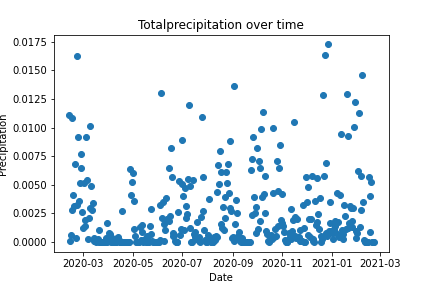
\includegraphics[width=.7\textwidth]{Figures/precipitation.png}


\subsection{Folium maps}
Furthermore, we created choropleths of hospitalized addition, population, and cases per capita based on the regions of the Netherlands. The figure below is a choropleth of cases per capita of the regions which illustrates that Rotterdam and the Hague were the most affected regions.



\includegraphics[width=.7\textwidth]{Figures/map.png}


\subsection{Pearson and Spearman correlation}
Moreover, we applied Pearson correlation to find the quantitative representations of the correlations between the corona data and weather variables, specifically between the cases per region and total precipitation variables. From our results, we were able to gather that the temperature above ground variable has the most statistical significance in regards to the p-value and also has the highest absolute value amongst the coefficients of all the weather variables used in the Pearson correlation test. On the other hand, total precipitation does not appear to have a significant correlation with corona outbreaks as shown by the Pearson correlation coefficient.

Likewise, the Spearman correlation test showed us similar results, i.e., temperature above ground has the highest absolute value of coefficient along with the lowest p-value indicating high statistical significance once again. In fact, the p-value is 0.0 which is exceptionally good, indicating that the null hypothesis is entirely rejected, which could either be a coincidence or a computational mistake. The coefficient has also increased relatively indicating a stronger correlation between the variables. The absolute value of Spearman's correlation coefficient of the total precipitation decreased to 0.073 compared to Pearson's correlation coefficient of 0.077, whereas the p-value increased indicating a decrease in statistical significance. The negative coefficient indicates a decreasing monotonic trend between corona cases per region and total precipitation.

The results gathered from the Bonferroni and Holm-Bonferroni corrections returned true for total precipitation which implies that the p values are below the threshold of 0.005 further indicating that total precipitation is statistically significant with regards to the corona outbreak intensity.

\subsection{OLS regression results}
In addition, we also performed Ordinary Least Squares (OLS) regression on our dataset. We used cases per region as our dependent variable and the weather variables as our independent variables. The result showed us that total precipitation had the highest coefficient of 0.0001 and a relatively low standard error. Moreover, we also looked at the logged OLS regression and found exactly the same results for the same variables.

\subsection{OLS regression of dataframe merged with stringency index data}
For the OLS merged with the stringency index, the total precipitation has a coefficient of 1.907e-06 which is relatively high compared to the other weather factors. However, it also has a quite high standard error of 3e-05. The lowest coefficient is -7.163e-17 for the “International Support” factor. The highest coefficient is international travel controls with the value 7.047e-06.
\section{Discussion}

The results for the different weather factors were somewhat contradictory.

The results of the Pearson correlation showed that the temperature above ground is the most statistically significant according to the Pearson correlation.

Whereas the OLS regression models including the regression merged with stringency index data show that total precipitation has the strongest correlation with total precipitation from the weather variables. The Bonferroni and Holm-Bonferroni returned "True" for total precipitation showcasing that it is indeed statistically significant with respect to cases per region. 

According to the analysis that we carried out on the provided data sets, total precipitation also has a strong correlation with our dependent variable.

A research paper \citep{Menebo2020} that researched temperature and precipitation associated with Covid-19, based in Oslo, Norway. The paper aimed at analyzing the correlation between weather and corona data. The results of their research showed that temperature and precipitation are associated with daily corona cases. This reflects our hypothesis. Temperature was positively associated with corona whereas precipitation is negatively related.

A hypothesis for the correlation of total precipitation to corona is when precipitation is high, people tend to stay inside due to the rain, snow, or other environmental factors while still going to work, school, or holding social gatherings indoors. By doing so, they tend to be close together with friends and family where air circulation is undesirable, meaning the spread of corona could be intensified.

Another hypothesis is that low precipitation enables people to spend more time outside allowing people to break restrictions and be exposed to the virus.

Both of the above hypotheses do not actually prove direct causation between the temperature above ground, precipitation, or other environmental factors and the spread of the virus. It can be noted that the environmental factors changing human behavior to that of them to having more social interactions carry an increased risk of virus transmission, but it does not actually create a biologically beneficial environment for the spread of the virus.

\section{Limitations}

During the research we encountered several obstacles that could be a deterring factor in the validity of our results. Firstly, the analysed data set lacked the number of covid tests carried out. This could potentially make the number of cases irrelevant. However, the number of deaths and hospitalizations remain an objective indicator that is independent of the missing values. 

Some of the values were dropped during the merging of data due to technicalities. This could have a negative impact on the scope of data. Specifically, 204 rows of the original data set were dropped. 

Another issue we stumbled upon were the missing values in stringency index, which might limit the accuracy of the measurements that we used to correlate the measure of covid cases and the environmental factors. % If we're not doing anything with regards to the Government Interventions in the report, then this is not a limitation. 

Finally, we didn't have any information regarding government regulations introduced during the outbreaks of covid, such as lockdowns, which could limit the exposure of people to environmental factors. % Perhaps reword to be more along the lines of: "Finally, we didn't adjust for external interventions, eg. Government Interventions, which could also play a role. 

\section{Concluding Remarks}

The results from the research suggest a possible correlation between the corona outbreaks with the temperature above the ground variable along with a possible correlation with the total precipitation variable. Although total precipitation has a significant impact on the cases per region, we observed that the temperature above ground impacted the variable more according to the Pearson correlation. On the contrary,  every result pointed to total precipitation as the most correlated variable confirming our hypothesis. However, it is likely that the weather only impacts the social behavior of people in the Netherlands and does not actually provide a better environment for the spread of the virus. It is important to note that our research has many limitations, hence we do not recommend our results to be used for any further research.

Research conducted is not completely flawless, so its findings should be taken into account with careful consideration. The future works in this area can be based on the coefficients describing the relationship between weather as well as inspecting the unconsidered factors such as humidity.

% \section{Disclosure Statement}




%-------------------------------------------------------------------------------
% REFERENCES
%-------------------------------------------------------------------------------
\newpage
\addcontentsline{toc}{section}{References}
\bibliography{bib}
\appendix

\begin{landscape}
\newpage

\section{Tables}
\subsection{Weather Data metrics}
\begin{tabular}{lrrrrrrrr}
\toprule
Variable &    count &          mean &           std &           min &           25\% &           50\% &           75\% &           max \\
\midrule
RelativeHumiditySurface &  20220.0 &  7.70e+01 &  1.31e+01 &  3.38e+01 &  6.78e+01 &  7.93e+01 &  8.78e+01 &  9.90e+01 \\
SolarRadiation          &  20220.0 &  6.41e+06 &  6.32e+06 &  0.00e+00 &  7.78e+05 &  4.16e+06 &  1.11e+07 &  2.48e+07 \\
Surfacepressure         &  20220.0 &  2.39e+06 &  5.03e+04 &  2.18e+06 &  2.36e+06 &  2.40e+06 &  2.43e+06 &  2.49e+06 \\
TemperatureAboveGround  &  20220.0 &  2.81e+02 &  7.58e+00 &  2.50e+02 &  2.76e+02 &  2.82e+02 &  2.87e+02 &  3.01e+02 \\
Totalprecipitation      &  20220.0 &  2.20e-03 &  3.39e-03 &  0.00e+00 &  7.20e-05 &  7.20e-04 &  2.90e-03 &  4.13e-02 \\
UVIndex                 &  20220.0 &  1.42e+01 &  1.39e+01 &  0.00e+00 &  3.38e-01 &  9.75e+00 &  2.55e+01 &  5.27e+01 \\
WindSpeed               &  20220.0 &  3.72e+00 &  1.74e+00 &  6.87e-01 &  2.44e+00 &  3.33e+00 &  4.61e+00 &  1.37e+01 \\
\bottomrule
\end{tabular}


\subsection{Corona Data metrics}
\begin{tabular}{lrrrrrrrr}
\toprule
{} &   count &          mean &           std &   min &     25\% &     50\% &       75\% &       max \\
\midrule
region\_code             &  4344.0 &     25.500000 &      3.452450 &  20.0 &   22.75 &    25.5 &     28.25 &      31.0 \\
deceased\_addition       &  4152.0 &      3.665703 &      6.923995 &  -3.0 &    0.00 &     1.0 &      4.00 &      77.0 \\
confirmed\_addition      &  4332.0 &    244.049400 &    417.929016 & -46.0 &    8.00 &    68.0 &    257.00 &    3179.0 \\
hospitalized\_addition   &  4152.0 &      5.698940 &     12.976320 &  -3.0 &    0.00 &     1.0 &      6.00 &     270.0 \\
deceased\_cumulative     &  4164.0 &    605.770653 &    692.735743 &   0.0 &   69.00 &   314.0 &    870.25 &    3653.0 \\
confirmed\_cumulative    &  4344.0 &  23076.545580 &  42795.712372 &   0.0 &  936.00 &  6088.0 &  18962.75 &  250759.0 \\
hospitalized\_cumulative &  4164.0 &   1144.249039 &   1179.334164 &   0.0 &  161.00 &   619.0 &   1749.50 &    6043.0 \\
\bottomrule
\end{tabular}

\end{landscape}

\newpage
\section{Correlations}
\subsection{Pearson}
\begin{tabular}{lrr}
\toprule
{} &   Correlation &  p-values \\
\midrule
RelativeHumiditySurface &  3.429129e-16 & -0.126307 \\
SolarRadiation          &  5.628132e-01 &  0.008996 \\
Surfacepressure         &  1.971974e-10 &  0.098688 \\
TemperatureAboveGround  &  1.496281e-43 & -0.212671 \\
Totalprecipitation      &  1.599316e-05 & -0.067000 \\
UVIndex                 &  5.656131e-26 & -0.162764 \\
WindSpeed               &  5.808188e-04 &  0.053448 \\
\bottomrule
\end{tabular}


\subsection{Spearman}
\begin{tabular}{lrr}
\toprule
{} &    Correlation &  p-values \\
\midrule
RelativeHumiditySurface &   3.268932e-15 &  0.122051 \\
SolarRadiation          &   6.749240e-57 & -0.243401 \\
Surfacepressure         &   1.143578e-01 &  0.024543 \\
TemperatureAboveGround  &  7.826975e-256 & -0.495802 \\
Totalprecipitation      &   8.558288e-05 & -0.061013 \\
UVIndex                 &  1.872523e-210 & -0.454739 \\
WindSpeed               &   1.972349e-10 &  0.098688 \\
\bottomrule
\end{tabular}


\end{document}
